
\documentclass[letterpaper,hide notes,xcolor={table,svgnames},pdftex]{beamer}
\def\showexamples{t}


%\usepackage[svgnames]{xcolor}

%% Demo talk
%\documentclass[letterpaper,notes=show]{beamer}

\usecolortheme{crane}
\setbeamertemplate{navigation symbols}{}

\usetheme{MyPittsburgh}
%\usetheme{Frankfurt}

%\usepackage{tipa}

\usepackage{hyperref}
\usepackage{graphicx,xspace}
\usepackage[normalem]{ulem}

\newcommand\SF[1]{$\bigstar$\footnote{SF: #1}}



\newcounter{tmpnumSlide}
\newcounter{tmpnumNote}

% old question code
%\newcommand\question[1]{{$\bigstar$ \small \onlySlide{2}{#1}}}
% \newcommand\nquestion[1]{\ifdefined \presentationonly \textcircled{?} \fi \note{\par{\Large \textbf{?}} #1}}
% \newcommand\nanswer[1]{\note{\par{\Large \textbf{A}} #1}}


 \newcommand\mnote[1]{%
   \addtocounter{tmpnumSlide}{1}
   \ifdefined\showcues {~\tiny\fbox{\arabic{tmpnumSlide}}}\fi
   \note{\setlength{\parskip}{1ex}\addtocounter{tmpnumNote}{1}\textbf{\Large \arabic{tmpnumNote}:} {#1\par}}}

\newcommand\mmnote[1]{\note{\setlength{\parskip}{1ex}#1\par}}

%\newcommand\mnote[2][]{\ifdefined\handoutwithnotes {~\tiny\fbox{#1}}\fi
% \note{\setlength{\parskip}{1ex}\textbf{\Large #1:} #2\par}}

%\newcommand\mnote[2][]{{\tiny\fbox{#1}} \note{\setlength{\parskip}{1ex}\textbf{\Large #1:} #2\par}}

\newcommand\mquestion[2]{{~\color{red}\fbox{?}}\note{\setlength{\parskip}{1ex}\par{\Large \textbf{?}} #1} \note{\setlength{\parskip}{1ex}\par{\Large \textbf{A}} #2\par}\ifdefined \presentationonly \pause \fi}

\newcommand\blackboard[1]{%
\ifdefined   \showblackboard
  {#1}
  \else {\begin{center} \fbox{\colorbox{blue!30}{%
         \begin{minipage}{.95\linewidth}%
           \hspace{\stretch{1}} Some space intentionally left blank; done at the blackboard.%
         \end{minipage}}}\end{center}}%
         \fi%
}



%\newcommand\q{\tikz \node[thick,color=black,shape=circle]{?};}
%\newcommand\q{\ifdefined \presentationonly \textcircled{?} \fi}

\usepackage{listings}
\lstset{%
  keywordstyle=\bfseries,
  aboveskip=15pt,
  belowskip=15pt,
  captionpos=b,
  identifierstyle=\ttfamily,
  escapeinside={(*@}{@*)},
  stringstyle=\ttfamiliy,
  frame=lines,
  numbers=left, basicstyle=\scriptsize, numberstyle=\tiny, stepnumber=0, numbersep=2pt}

\usepackage{siunitx}
\newcommand\sius[1]{\num[group-separator = {,}]{#1}\si{\micro\second}}
\newcommand\sims[1]{\num[group-separator = {,}]{#1}\si{\milli\second}}
\newcommand\sins[1]{\num[group-separator = {,}]{#1}\si{\nano\second}}
\sisetup{group-separator = {,}, group-digits = true}

%% -------------------- tikz --------------------
\usepackage{tikz}
\usetikzlibrary{positioning}
\usetikzlibrary{arrows,backgrounds,automata,decorations.shapes,decorations.pathmorphing,decorations.markings,decorations.text}

\tikzstyle{place}=[circle,draw=blue!50,fill=blue!20,thick, inner sep=0pt,minimum size=6mm]
\tikzstyle{transition}=[rectangle,draw=black!50,fill=black!20,thick, inner sep=0pt,minimum size=4mm]

\tikzstyle{block}=[rectangle,draw=black, thick, inner sep=5pt]
\tikzstyle{bullet}=[circle,draw=black, fill=black, thin, inner sep=2pt]

\tikzstyle{pre}=[<-,shorten <=1pt,>=stealth',semithick]
\tikzstyle{post}=[->,shorten >=1pt,>=stealth',semithick]
\tikzstyle{bi}=[<->,shorten >=1pt,shorten <=1pt, >=stealth',semithick]

\tikzstyle{mut}=[-,>=stealth',semithick]

\tikzstyle{treereset}=[dashed,->, shorten >=1pt,>=stealth',thin]

\usepackage{ifmtarg}
\usepackage{xifthen}
\makeatletter
% new counter to now which frame it is within the sequence
\newcounter{multiframecounter}
% initialize buffer for previously used frame title
\gdef\lastframetitle{\textit{undefined}}
% new environment for a multi-frame
\newenvironment{multiframe}[1][]{%
\ifthenelse{\isempty{#1}}{%
% if no frame title was set via optional parameter,
% only increase sequence counter by 1
\addtocounter{multiframecounter}{1}%
}{%
% new frame title has been provided, thus
% reset sequence counter to 1 and buffer frame title for later use
\setcounter{multiframecounter}{1}%
\gdef\lastframetitle{#1}%
}%
% start conventional frame environment and
% automatically set frame title followed by sequence counter
\begin{frame}%
\frametitle{\lastframetitle~{\normalfont(\arabic{multiframecounter})}}%
}{%
\end{frame}%
}
\makeatother

\makeatletter
\newdimen\tu@tmpa%
\newdimen\ydiffl%
\newdimen\xdiffl%
\newcommand\ydiff[2]{%
    \coordinate (tmpnamea) at (#1);%
    \coordinate (tmpnameb) at (#2);%
    \pgfextracty{\tu@tmpa}{\pgfpointanchor{tmpnamea}{center}}%
    \pgfextracty{\ydiffl}{\pgfpointanchor{tmpnameb}{center}}%
    \advance\ydiffl by -\tu@tmpa%
}
\newcommand\xdiff[2]{%
    \coordinate (tmpnamea) at (#1);%
    \coordinate (tmpnameb) at (#2);%
    \pgfextractx{\tu@tmpa}{\pgfpointanchor{tmpnamea}{center}}%
    \pgfextractx{\xdiffl}{\pgfpointanchor{tmpnameb}{center}}%
    \advance\xdiffl by -\tu@tmpa%
}
\makeatother
\newcommand{\copyrightbox}[3][r]{%
\begin{tikzpicture}%
\node[inner sep=0pt,minimum size=2em](ciimage){#2};
\usefont{OT1}{phv}{n}{n}\fontsize{4}{4}\selectfont
\ydiff{ciimage.south}{ciimage.north}
\xdiff{ciimage.west}{ciimage.east}
\ifthenelse{\equal{#1}{r}}{%
\node[inner sep=0pt,right=1ex of ciimage.south east,anchor=north west,rotate=90]%
{\raggedleft\color{black!50}\parbox{\the\ydiffl}{\raggedright{}#3}};%
}{%
\ifthenelse{\equal{#1}{l}}{%
\node[inner sep=0pt,right=1ex of ciimage.south west,anchor=south west,rotate=90]%
{\raggedleft\color{black!50}\parbox{\the\ydiffl}{\raggedright{}#3}};%
}{%
\node[inner sep=0pt,below=1ex of ciimage.south west,anchor=north west]%
{\raggedleft\color{black!50}\parbox{\the\xdiffl}{\raggedright{}#3}};%
}
}
\end{tikzpicture}
}


%% --------------------

%\usepackage[excludeor]{everyhook}
%\PushPreHook{par}{\setbox0=\lastbox\llap{MUH}}\box0}

%\vspace*{\stretch{1}

%\setbox0=\lastbox \llap{\textbullet\enskip}\box0}

\setlength{\parskip}{\fill}

\newcommand\noskips{\setlength{\parskip}{1ex}}
\newcommand\doskips{\setlength{\parskip}{\fill}}

\newcommand\xx{\par\vspace*{\stretch{1}}\par}
\newcommand\xxs{\par\vspace*{2ex}\par}
\newcommand\tuple[1]{\langle #1 \rangle}
\newcommand\code[1]{{\sf \footnotesize #1}}
\newcommand\ex[1]{\uline{Example:} \ifdefined \presentationonly \pause \fi
  \ifdefined\showexamples#1\xspace\else{\uline{\hspace*{2cm}}}\fi}

\newcommand\ceil[1]{\lceil #1 \rceil}


\AtBeginSection[]
{
   \begin{frame}
       \frametitle{Outline}
       \tableofcontents[currentsection]
   \end{frame}
}



\pgfdeclarelayer{edgelayer}
\pgfdeclarelayer{nodelayer}
\pgfsetlayers{edgelayer,nodelayer,main}

\tikzstyle{none}=[inner sep=0pt]
\tikzstyle{rn}=[circle,fill=Red,draw=Black,line width=0.8 pt]
\tikzstyle{gn}=[circle,fill=Lime,draw=Black,line width=0.8 pt]
\tikzstyle{yn}=[circle,fill=Yellow,draw=Black,line width=0.8 pt]
\tikzstyle{empty}=[circle,fill=White,draw=Black]
\tikzstyle{bw} = [rectangle, draw, fill=blue!20, 
    text width=4em, text centered, rounded corners, minimum height=2em]
    
    \newcommand{\CcNote}[1]{% longname
	This work is licensed under the \textit{Creative Commons #1 3.0 License}.%
}
\newcommand{\CcImageBy}[1]{%
	\includegraphics[scale=#1]{creative_commons/cc_by_30.pdf}%
}
\newcommand{\CcImageSa}[1]{%
	\includegraphics[scale=#1]{creative_commons/cc_sa_30.pdf}%
}
\newcommand{\CcImageNc}[1]{%
	\includegraphics[scale=#1]{creative_commons/cc_nc_30.pdf}%
}
\newcommand{\CcGroupBySa}[2]{% zoom, gap
	\CcImageBy{#1}\hspace*{#2}\CcImageNc{#1}\hspace*{#2}\CcImageSa{#1}%
}
\newcommand{\CcLongnameByNcSa}{Attribution-NonCommercial-ShareAlike}

\newenvironment{changemargin}[1]{% 
  \begin{list}{}{% 
    \setlength{\topsep}{0pt}% 
    \setlength{\leftmargin}{#1}% 
    \setlength{\rightmargin}{1em}
    \setlength{\listparindent}{\parindent}% 
    \setlength{\itemindent}{\parindent}% 
    \setlength{\parsep}{\parskip}% 
  }% 
  \item[]}{\end{list}} 




\usepackage{alltt}

\title{Lecture 3 --- Java II}

\author{Patrick Lam \& Jeff Zarnett \\ \small \texttt{p.lam@ece.uwaterloo.ca} \& \texttt{jzarnett@uwaterloo.ca}}
\institute{Department of Electrical and Computer Engineering \\
  University of Waterloo}
\date{\today}


\begin{document}


\begin{frame}
  \titlepage
\end{frame}

\begin{frame}
\frametitle{Refresher: Object-oriented Programming}

\large
\begin{changemargin}{1.5cm}
Fundamental idea: use ``objects'' to encapsulate data.\vfill

Instantiate new objects with the \texttt{new} keyword.

{\tt class\footnote{Java doesn't have {\tt struct}.} Point \{ int x, y; \} }\vfill
{\tt Point p = new Point(); }
\end{changemargin}

\end{frame}

\begin{frame}
\frametitle{Classes versus Instances}

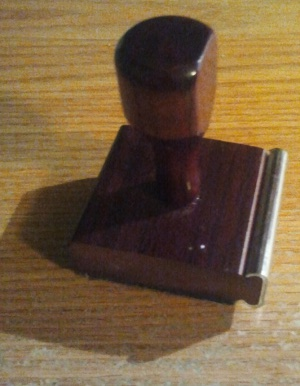
\includegraphics[width=.45\textwidth]{images/peo-stamp-small.jpg}

\includegraphics[width=.45\textwidth]{images/1502_cookies.jpg}

\begin{center}
Which is the class? Which is the instance?
\end{center}

\end{frame}

\begin{frame}
\frametitle{Classes and Relations}
\begin{changemargin}{1cm}
Java, like C\#, has \textit{inheritance}.

$B$ \underline{inherits} from $A$ if $B$ \texttt{extends} $A$ by using (at least some of) its methods and fields in addition to any of its own.

$B$ is a ``subclass'' or ``child'' of $A$

$A$ is a ``superclass'' or ``parent'' of $B$.

In this class we'll use the subclass/superclass terminology.
\end{changemargin}
\end{frame}

\begin{frame}
\frametitle{Class Hierarchy}
\begin{changemargin}{1cm}
In Java, all classes have a single inheritance hierarchy: each class has exactly one superclass. 

(Other languages like C++ allow multiple inheritance) 

The keyword in Java for declaring a class as a subclass of another is \texttt{extends}.

For example: \texttt{public class Book extends Document}

\end{changemargin}
\end{frame}

\begin{frame}
\frametitle{Class Hierarchy}
\begin{changemargin}{1cm}
Every object in Java eventually descends from \texttt{Object}.

If you do not declare a specific superclass with the \texttt{extends} keyword, the superclass will be \texttt{Object}.
\end{changemargin}
\end{frame}

\begin{frame}
\frametitle{Subclassing Example}

\begin{center}
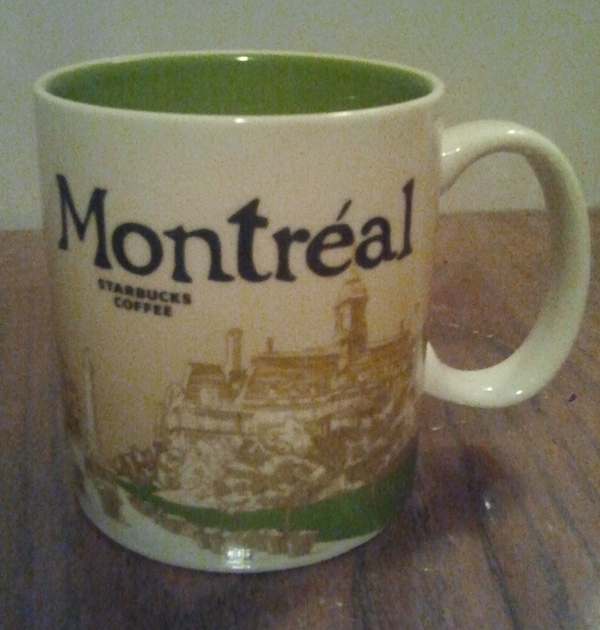
\includegraphics[width=.3\textwidth]{images/mug-scaled}
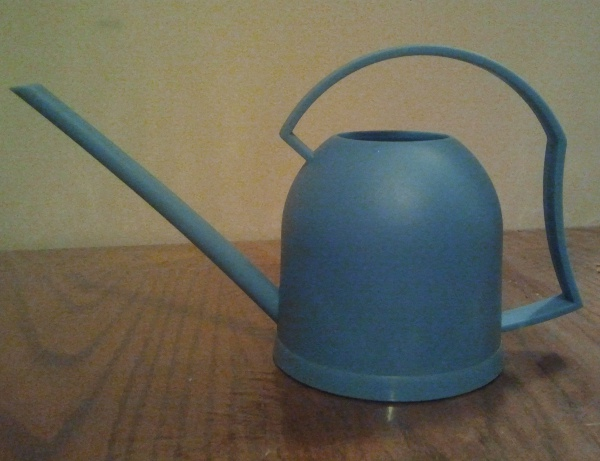
\includegraphics[width=.41\textwidth]{images/wateringcan-scaled.jpg}
\end{center}

\begin{alltt}
  class Mug \alert{extends} Donut \{ ... \}\\
  class WateringCan \alert{extends} Donut \{ ... \}
\end{alltt}

\end{frame}

\begin{frame}
\frametitle{Conceptual Meaning of Subclassing}

\begin{center}
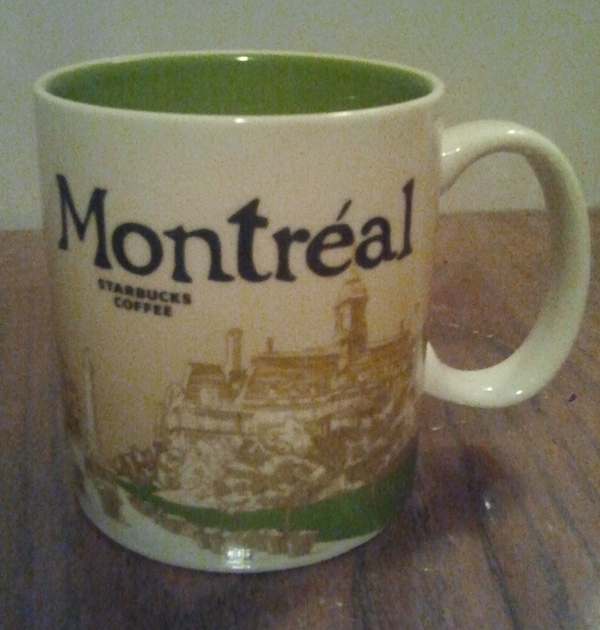
\includegraphics[width=.3\textwidth]{images/mug-scaled}
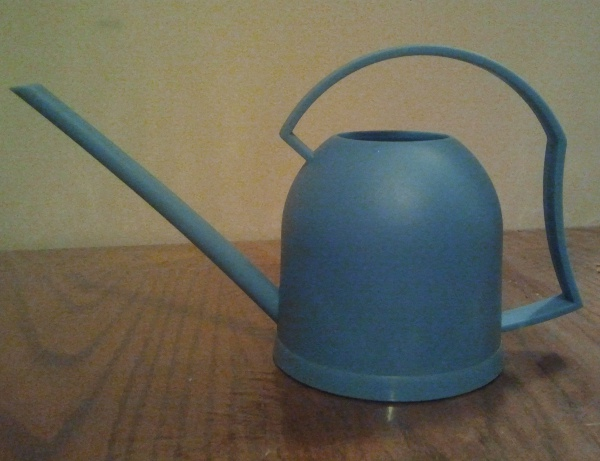
\includegraphics[width=.41\textwidth]{images/wateringcan-scaled.jpg}
\end{center}
\begin{alltt}
  class Mug extends Donut \{ ... \}\\
  class WateringCan extends Donut \{ ... \}
\end{alltt}

\begin{changemargin}{1.5cm}
\alert{\Large Subclassing encodes the ``is-a'' relationship.}
\end{changemargin}

\end{frame}

\begin{frame}
\frametitle{Advantages of Sucblassing}
\begin{changemargin}{1cm}
Avoiding repetition: don't re-implement code that is common.

\textit{Polymorphism} -- the ability of a class to look like another. 

Example: method expects \texttt{Rectangle}. You can use it on a \texttt{Square} and it will work if \texttt{Square extends Rectangle}.
\end{changemargin}
\end{frame}

\begin{frame}
\frametitle{Subclassing Calling Semantics}
\begin{changemargin}{1cm}

On (or inside of) a subclass we can call a method of the parent class. 

\texttt{Book} descends from \texttt{Object}, either directly or indirectly. 

Given that \texttt{toString()} is defined on \texttt{Object}, we can call the \texttt{toString()} method on a \texttt{Book}.

\end{changemargin}
\end{frame}

\begin{frame}
\frametitle{Subclassing Calling Semantics}
\begin{changemargin}{1cm}

Also from within a subclass, we can use an implementation of a method from a parent class with the keyword \texttt{super}.

The most common situation where this happens is in the constructor. 
\end{changemargin}
\end{frame}

\begin{frame}[fragile]
\frametitle{Subclassing Calling Semantics}
\begin{changemargin}{1cm}
{\scriptsize
\begin{verbatim}
public class Book extends Document {

  public Book() {
    super();
    setPageWidthInCm(20);
    setPageHeightInCm(30);
  }
  
  ...
}
public class Document implements Readable

  public Document() {
    setRead(false);
    setTitle(``Untitled'');
    setAuthor(Environment.getUserID());
  }
  
  ...
}
\end{verbatim}
}
\end{changemargin}
\end{frame}


\begin{frame}
\frametitle{\texttt{static}}
\begin{changemargin}{1cm}
When you see the keyword \texttt{static}, it is a modifier that means there is only one copy of the thing. 

\texttt{main()} in Java is declared as \texttt{static}; \\
\quad declare variables as \texttt{static} to reference them in \texttt{main}. 

Let's examine the semantics of this keyword.
\end{changemargin}
\end{frame}

\begin{frame}
\frametitle{Static Variable}
\begin{changemargin}{1cm}

The variable is common to all instances of a class. 

Assume you have an integer \texttt{i} in class $A$ and there are two instances of the class called $A_{1}$ and $A_{2}$. 

The value of \texttt{i} is the same and shared between $A_{1}$ and $A_{2}$.

A common variable can  keep a running total of the number of times a method has been called.
\end{changemargin}
\end{frame}

\begin{frame}
\frametitle{Static Method}
\begin{changemargin}{1cm}

The method is shared between all instances of the class. 

Cannot access instance variables/methods of the class\\
\quad only methods and variables that share the static modifier.

\end{changemargin}
\end{frame}

\begin{frame}
\frametitle{Static Class}
\begin{changemargin}{1cm}

The modifier cannot be applied to a class. 

There are a number of useful Java classes which offer their functionality only in \texttt{static} methods, such as the \texttt{Math} class. 

Using \texttt{Math} you can perform such operations as square root.

It doesn't make logical sense to instantiate \texttt{new Math()} to perform such an operation. 

\end{changemargin}
\end{frame}


\begin{frame}
\frametitle{Interfaces}
\only<1>{One of these things is not like the others:}
\only<2>{All but one of these things implement the {\tt HasHandle} interface.}

\begin{center}
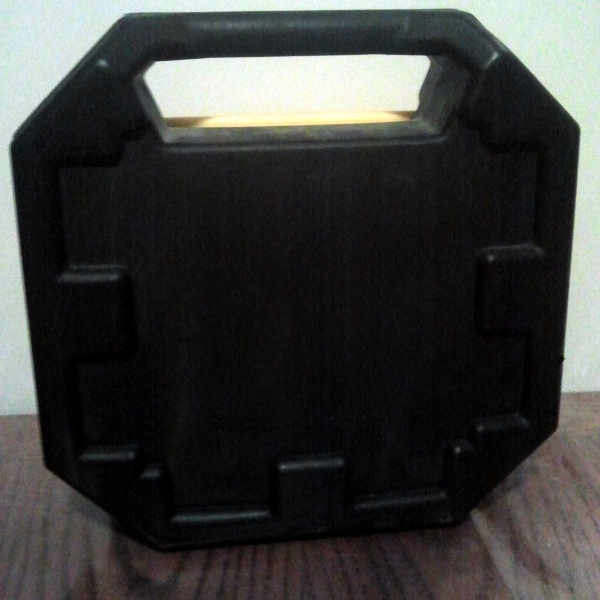
\includegraphics[width=.31\textwidth]{images/box-scaled.jpg}
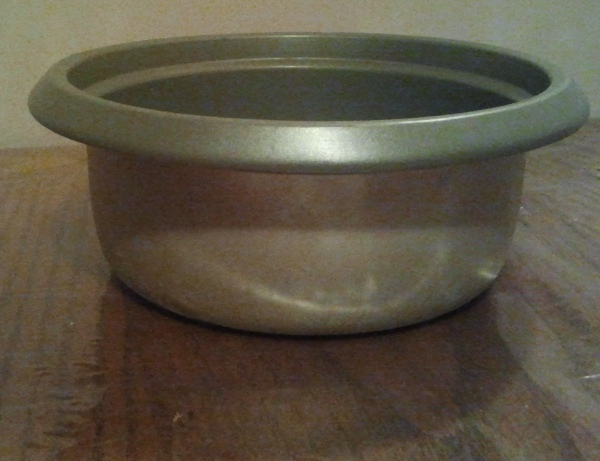
\includegraphics[width=.4\textwidth]{images/bowl-scaled.jpg}\\
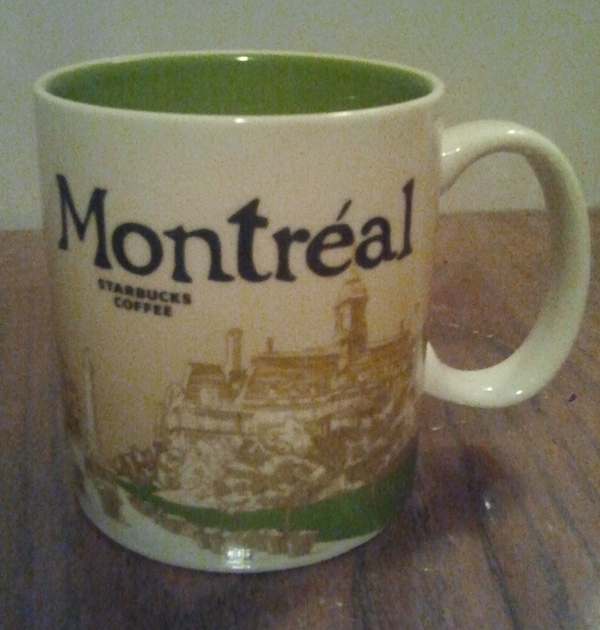
\includegraphics[width=.3\textwidth]{images/mug-scaled}
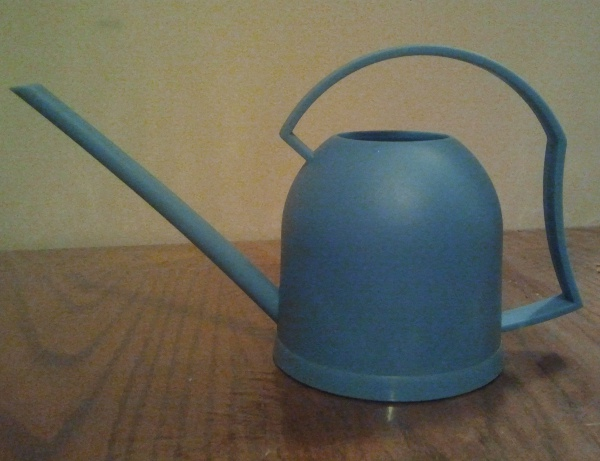
\includegraphics[width=.41\textwidth]{images/wateringcan-scaled.jpg}
\end{center}

\end{frame}

\begin{frame}
\frametitle{Using Interfaces}

\begin{changemargin}{2.5cm}
\begin{alltt}
  interface HasHandle \{ \\
\qquad    void pickup(); \\
  \}\\[1em]
  class Donut \alert{implements} HasHandle \{ \\
\qquad    void pickup() \{ \ldots~\}  \\
\qquad    \ldots \\
  \}\\
\end{alltt}
\end{changemargin}

\end{frame}

\begin{frame}
\frametitle{Interfaces as Contracts}
\begin{changemargin}{1cm}

An \texttt{interface} is a way of specifying in Java what is effectively a contract. 

The interface specifies some number of methods which any class that wants to implement this interface must have.

\end{changemargin}
\end{frame}


\begin{frame}[fragile]
\frametitle{Interfaces as Contracts}
\begin{changemargin}{1cm}

\begin{verbatim}
public interface Drawable {
  void draw();
}
\end{verbatim}

Any class which implements \texttt{Drawable} must contain an implementation of the method \texttt{draw()}.

\end{changemargin}
\end{frame}

\begin{frame}
\frametitle{Interface Semantics}
\begin{changemargin}{1cm}

Methods that are declared in an interface are always public.\\
\quad Other modifiers are not allowed.

Interfaces can extend other interfaces, but may never contain implementation. 

An interface may declare some constants.

Accordingly, an interface can never be instantiated. 

A class can implement as many interfaces as desired.

\end{changemargin}
\end{frame}

\begin{frame}
\frametitle{Why Interfaces?}
\begin{changemargin}{1cm}

Interact with an object without knowing what it is underneath. 

Example: \texttt{Comparable} allows the JRE to sort objects.

For a built-in sort, the object must implement \texttt{Comparable}.\\\quad (otherwise Java has no idea how to order them). 

\texttt{Comparable}: only one method (\texttt{CompareTo}) is required.
\end{changemargin}
\end{frame}

\begin{frame}
\frametitle{Why Interfaces?}
\begin{changemargin}{1cm}

 If the objects we are looking at represent soccer players. 
 
 Sort them by their uniform numbers ascending. 
 
 Implement that logic in \texttt{CompareTo}. 
 
 Then we can use something like \texttt{Collections.sort()}. 
 
 The JRE sorts without having to know anything in advance about the soccer players.
\end{changemargin}
\end{frame}

\begin{frame}
\frametitle{Abstract Classes}
\begin{changemargin}{1cm}

Halfway between an interface and a regular class is the \alert{abstract class}. 

Declared using the \texttt{abstract} keyword. 

May (but does not have to) contain abstract methods. 

However, any class that contains methods marked \texttt{abstract} must also be marked as \texttt{abstract}. 

Cannot be instantiated, but may be subclassed. 

An abstract class can have as much or as little implementation as desired.
\end{changemargin}
\end{frame}

\begin{frame}[fragile]
\frametitle{Abstract Classes}
\begin{changemargin}{1cm}

To declare an abstract method, write the method signature, but with the keyword \texttt{abstract} attached: 

\verb+public abstract void draw(int parameter);+.


Abstract classes may have static fields and methods.\\
\quad e.g. \texttt{AbstractClass.method()}.


\end{changemargin}
\end{frame}

\begin{frame}
\frametitle{Abstract Classes vs. Interfaces}
\begin{changemargin}{1cm}

There are similarities between abstract classes \& interfaces.

When should each of these be used?

\end{changemargin}
\end{frame}

\begin{frame}
\frametitle{Use Abstract Class When}
\begin{changemargin}{1cm}

\begin{itemize}
\item To share code among several closely related classes.
\item Classes that extend your abstract class have many common methods or fields, or require access modifiers other than public (such as protected and private).
\item To declare non-static or non-final fields. 
\end{itemize}

\end{changemargin}
\end{frame}

\begin{frame}
\frametitle{Use Interface When}
\begin{changemargin}{1cm}

\begin{itemize}
\item Unrelated classes would implement your interface. 
\item You want to specify the behaviour of a particular data type, but not concerned about who implements its behaviour.
\item You want to take advantage of multiple inheritance of type (i.e. implement multiple interfaces on one class)
\end{itemize}

\end{changemargin}
\end{frame}

\begin{frame}
\frametitle{Why Not Both?}
\begin{changemargin}{1cm}

An interface can be partly implemented by an abstract class. 

The concrete class that extends the abstract class is responsible for implementing any of the methods of the interface that its superclass does not. 
\end{changemargin}
\end{frame}

\begin{frame}
\frametitle{Why Not Both?}
\begin{changemargin}{1cm}
Imagine interface $K$ has 4 methods. 

There is an abstract class $L$ declared as \texttt{implements K}. 

Suppose $L$ implements 3 of the 4 methods of $K$. 

When a subclass $P$ of $L$ is declared, then $P$ must implement that method that $L$ did not (or else be abstract itself).

\end{changemargin}
\end{frame}


\begin{frame}
\frametitle{Visibility Modifiers}
\begin{changemargin}{1cm}
There are four options for visibility (accessibility) of something (a variable, method, class, etc) declared outside of a function. 

\begin{itemize}
	\item \texttt{public}
	\item \texttt{private}
	\item \texttt{protected}
	\item \textit{(No Modifier)} Don't use this.
\end{itemize}

\end{changemargin}
\end{frame}

\begin{frame}
\frametitle{Visibility Modifiers: Why Bother?}
\begin{changemargin}{1cm}

Could one in theory just declare everything \texttt{public}? 

Probably, but it is very poor programming practice. 

Java convention: encapsulation and information hiding: the internal state of objects should not be visible to the world. 
\end{changemargin}
\end{frame}

\begin{frame}
\frametitle{Visibility Modifiers: Why Bother?}
\begin{changemargin}{1cm}
In the real world anything that is \texttt{public} will be accessed by other programmers. 

They may come to depend on a particular implementation detail (a problem that Microsoft has in abundance). 

Consider carefully if a method should be accessible from outside the given class.

If the answer is no, then \texttt{private} is the right answer for the modifier, or \texttt{protected} if it may be used in a subclass.
\end{changemargin}
\end{frame}


\begin{frame}
\frametitle{\texttt{final}}
\begin{changemargin}{1cm}
Another keyword: \texttt{final}. This can be applied to three things, with slightly different meanings:
\begin{itemize}
	\item Field
	\item Method
	\item Class
\end{itemize}
We cannot apply \texttt{final} to an interface, because we will obviously have to implement it somehow. 

Similarly, we cannot make an abstract class final, because it is meant to be subclassed. 

\end{changemargin}
\end{frame}

\begin{frame}
\frametitle{Worked Example: Shapes}
\begin{changemargin}{1cm}
Done on the board to facilitate understanding.

(See notes for full details)

\end{changemargin}
\end{frame}

\begin{frame}
\frametitle{Modifier Summary}

{\tiny
\begin{center}
\begin{tabular}{|p{1.5cm}|p{1cm}|p{1cm}|p{1cm}|p{1cm}|p{2cm}|}
\hline
\textbf{Modifier} & \textbf{Interface} & \textbf{Class} & \textbf{Nested Class} & \textbf{Field} & \textbf{Method} \\
\hline
\texttt{public} & \multicolumn{5}{l|}{Accessible from any class.}\\
\hline
\texttt{private} & \multicolumn{5}{l|}{Accessible only from this class.}\\
\hline
\texttt{protected} & \multicolumn{5}{l|}{Accessible only from this class and its subclasses.}\\
\hline
(No modifier) & \multicolumn{5}{l|}{Accessible from any class within the same package. Don't use this.}\\
\hline
\hline
\texttt{abstract} & N/A & \multicolumn{2}{p{4cm}|}{Contains at least one \texttt{abstract} method; cannot be instantiated.} & N/A & Its implementation is not defined; only signature \& return type declared.\\
\hline
\texttt{final} & N/A & \multicolumn{2}{l|}{Cannot be subclassed.} & Its value cannot be changed. & It cannot be overridden by a subclass. \\
\hline
\texttt{static} & N/A & N/A & Not an inner class. & Exactly one instance exists for all objects of the class. & Exactly one instance exists for all objects of the class. \\
\hline

\end{tabular}
\end{center}
}

\end{frame}

\end{document}

